\documentclass[autodetect-engine,dvipdfmx-if-dvi,ja=standard,everyparhook=compat]{bxjsarticle}

\usepackage{graphicx}        % 図を表示するのに必要
\usepackage{color}           % jpgなどを表示するのに必要
\usepackage{amsmath,amssymb} % 数学記号を出すのに必要
\usepackage{type1cm}         % fontsizeのエラー回避
\usepackage{here}            % 図の強制配置
\usepackage{url}             % URLをいい感じにしてくれる
\usepackage{subfigure}       % 図をまとめて表示
\usepackage{pdfpages}        % PDFの連結
\usepackage{setspace}
\usepackage{cases}
\usepackage{fancyhdr}
\usepackage{wrapfig}% 図の回り込み


% 余白の設定
% \setlength{\textheight}{\paperheight}   % 紙面縦幅を本文領域にする(BOTTOM=-TOP)
% \setlength{\topmargin}{-15.4truemm}     % 上の余白を10mm(=1inch-15.4mm)に
% \addtolength{\topmargin}{-\headheight}  %
% \addtolength{\topmargin}{-\headsep}     % ヘッダの分だけ本文領域を移動させる
% \addtolength{\textheight}{-20truemm}    % 下の余白も10mm
% \setlength{\textwidth}{\paperwidth}     % 紙面横幅を本文領域にする(RIGHT=-LEFT)
% \setlength{\oddsidemargin}{-5.4truemm}  % 奇数ページの左の余白を20mm(=1inch-5.4mm)に
% \setlength{\evensidemargin}{-5.4truemm} % 偶数数ページの左の余白を20mm(=1inch-5.4mm)に
% \addtolength{\textwidth}{-40truemm}     % 右の余白も20mm

% タイトル
\title{タイトル}

% ヘッダとフッタの設定
% \lhead{電気電子情報工学実験}
% \chead{}
% \rhead{20315784 佐藤凌雅}
% \lfoot{}
% \cfoot{\thepage} % ページ数
% \rfoot{}

\parindent = 0pt  % 行頭の字下げをしない
\setstretch{1.0}  % 行間

% キャプションの英語化
\renewcommand{\figurename}{Fig.}
\renewcommand{\tablename}{Table}

% 各章,節などタイトルの大きさを変更
% \titleformat*{\section}{\Huge\bfseries}
% \titleformat*{\subsection}{\Large\bfseries}

% 式の番号を(senction_num.num)のようにする
% \makeatletter
% \@addtoreset{equation}{chapter}
% \def\theequation{\thechapter.\arabic{equation}}
% \makeatother

% 呼び出したページのページ番号を消す
\newcommand{\deletePageNum}{
    \thispagestyle{empty}
    \clearpage
    \addtocounter{page}{-1}
}

% urlのフォントを直す
\renewcommand\UrlFont{\rmfamily}


\begin{document}
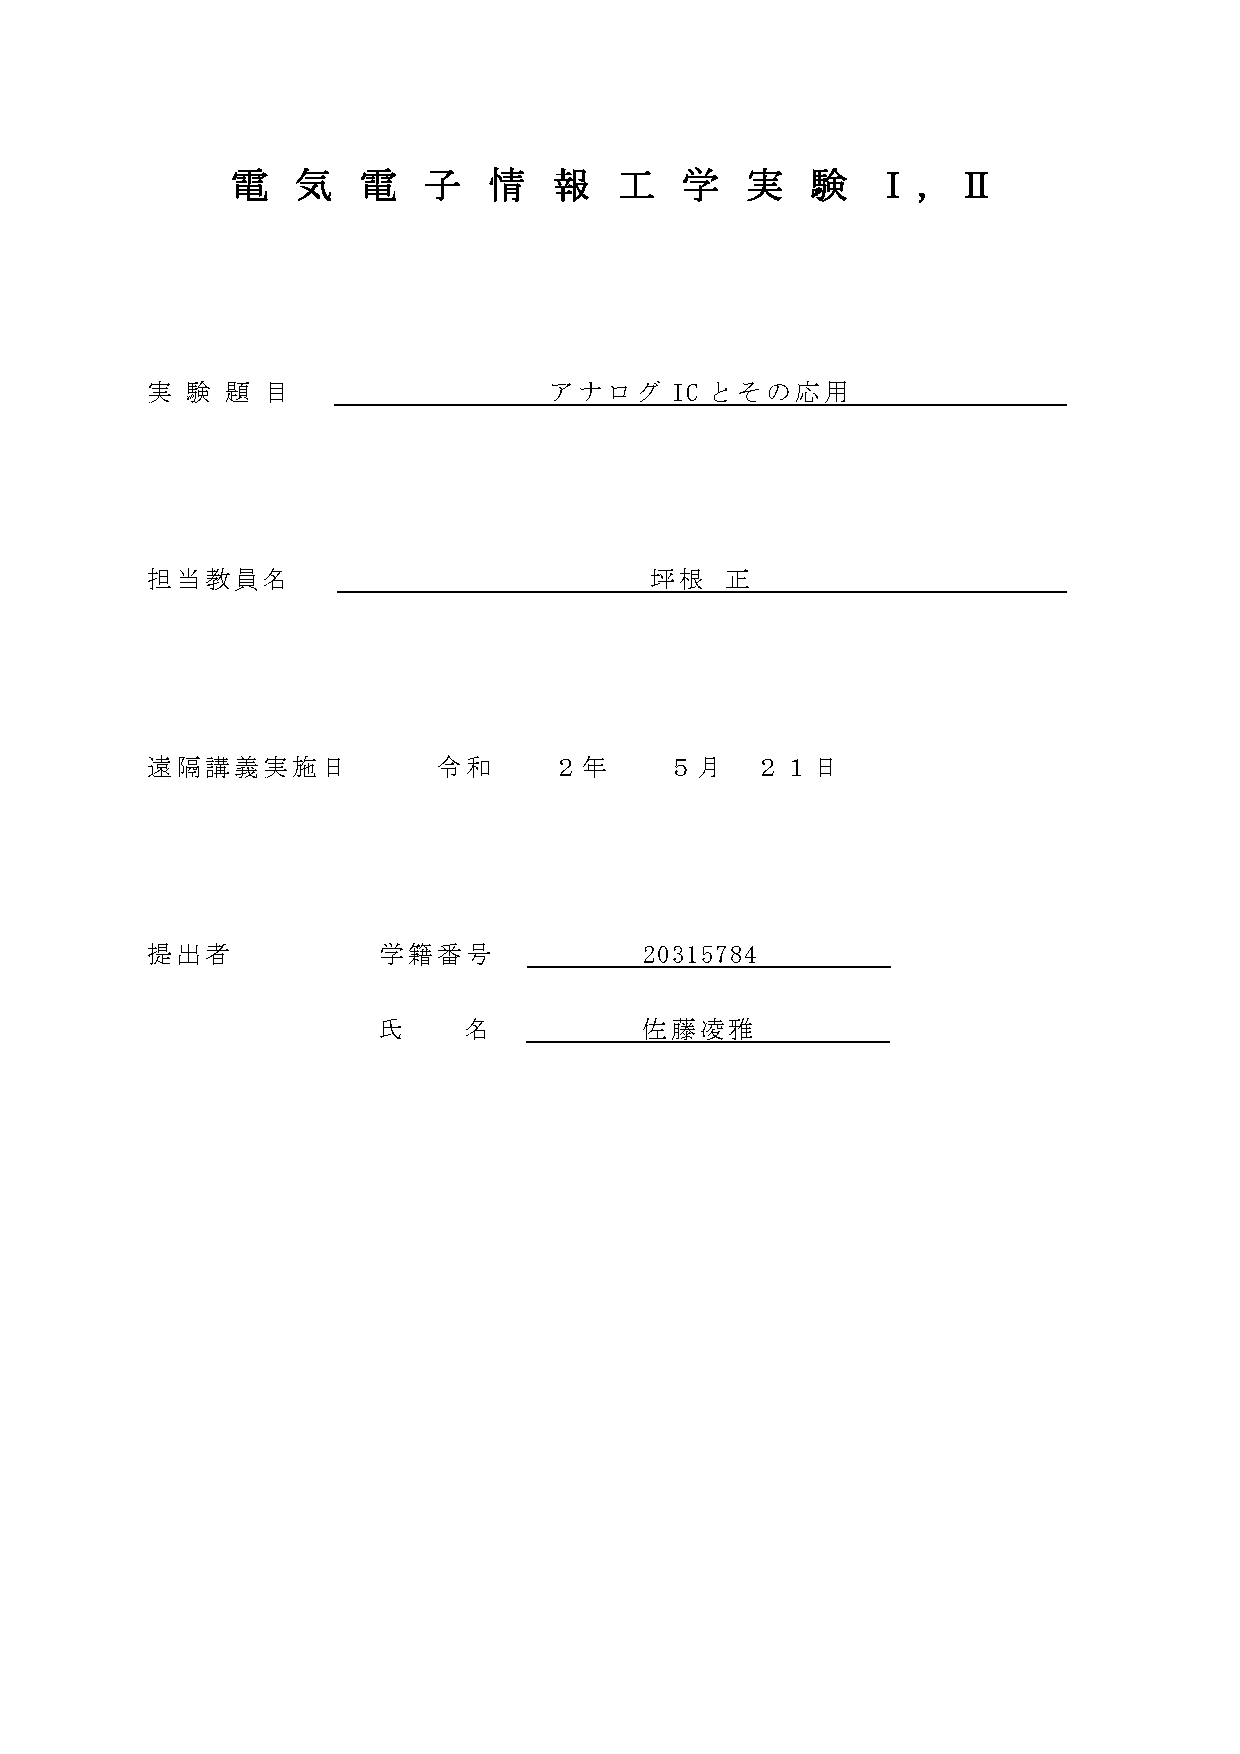
\includepdf[pages=-]{./setting/cover.pdf}
% \maketitle

\fontsize{11.041pt}{16.562pt}\selectfont

% 実験の目的,手段,結果,結論を簡潔にまとめ示すこと.(250字程度)
\section{概要 Abstract}

% テキストに書かれている目的等を参考に,各自どの点に注目して実験したのかを明確に示すこと.(300字程度)
\section{目的 Purpose}
 与えられた設計仕様を満たす2次低域通過フィルタと弛張発振器の作成を第一の目標と定める.要求された仕様を満たすことのできる回路を設計するため,2次低域通過フィルタでは,Q値およびカットオフ周波数と回路素子間の関係を数式で表現する.弛張発振器においても発振周波数と回路素子間の関係を導出する.いずれの回路においても最適な抵抗,キャパシタの値を理論に従って導出することで回路の設計を行う.さらに,導き出したパラメータを元に実際に回路を作成し,動作試験を行う.実験にて得られたデータを分析して与えられた設計仕様を満足しているかを確認し,それを考察する.


% 各自の実験目的に必要な理論的な背景を示すこと.必要ならば,参考文献リストより文献番号を引用すること.(レポート用紙1枚程度)
\section{理論的背景 Theory}
\subsection{2次低域通過フィルタの伝達関数}
 ここでは2次低域通過フィルタの伝達関数を導出する.2次低域通過フィルタの回路図をFig.\ref{fig:2D_LPF}に示す.
\begin{figure}[H]
    \centering
    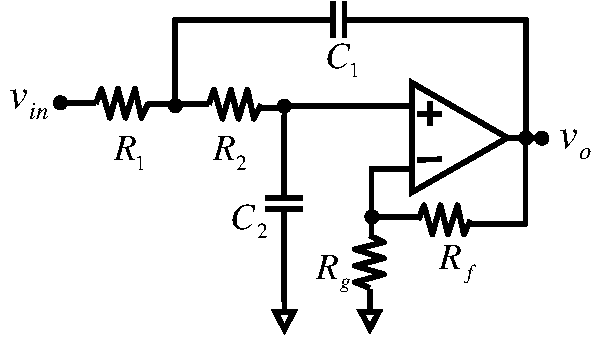
\includegraphics[scale=0.5]{./fig/2D_LPF.pdf}
    \caption{Second-order low-pass filter}
    \label{fig:2D_LPF}
\end{figure}


 この時,オペアンプと抵抗 $R_f$,$R_g$ で構成されているFig.\ref{fig:Non-inverting_amplifier}に示すような回路を非反転増幅器という.この回路は伝達関数は線形領域においてEqn.(\ref{eqn:transfer_function_Non-inverting_amplifier})となる.すなわち,抵抗 $R_f$,$R_g$ を調整することで,入力電圧を任意の定数($K$)倍する働きを持つと捉えることができる.
\begin{figure}[H]
    \centering
    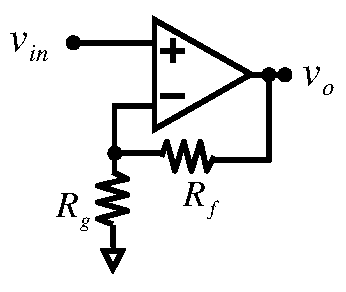
\includegraphics[scale=0.5]{./fig/Non-inverting_amplifier.pdf}
    \caption{Non-inverting amplifier}
    \label{fig:Non-inverting_amplifier}
\end{figure}

\begin{equation}
    \frac{v_{o}}{v_{i n}}=1+\frac{R_{f}}{R_{g}}=K
    \label{eqn:transfer_function_Non-inverting_amplifier}
\end{equation}

 これを踏まえて,$v_{i n}=R_{1}\left(i_{1}+i_{2}\right)+v_{1}$であることに留意し,2次低域通過フィルタの伝達関数を求めるとEqn.(\ref{eqn:transfer_function_2D_LPF})のようになる.
\begin{equation}
    \frac{v_{o}}{v_{i n}} = \frac{K \frac{1}{C_{1} C_{2} R_{1} R_{2}}}{s^{2}+\frac{1}{\sqrt{C_{1} C_{2} R_{1} R_{2}}}\{\sqrt{\frac{C_{2} R_{2}}{C_{1} R_{1}}}+\sqrt{\frac{C_{2} R_{1}}{C_{1} R_{2}}}+\sqrt{\frac{C_{1} R_{1}}{C_{2} R_{2}}}(1-K)\} s+\frac{1}{C_{1} C_{2} R_{1} R_{2}}}
    \label{eqn:transfer_function_2D_LPF}
\end{equation}

 ここで,双二次低域通過関数 $T_{LP}$ (Eqn(\ref{eqn:TLP}))と係数比較を行う.
\begin{equation}
    T_{L P}(s)=\frac{v_{o}}{v_{in}}=\frac{K \omega_{0}^{2}}{s^{2}+\frac{\omega_{0}}{Q} s+\omega_{0}^{2}}
    \label{eqn:TLP}
\end{equation}

 係数比較を行うと以下を得られる.
\begin{eqnarray}
    Q &=& \frac{1}{\sqrt{\frac{C_{2} R_{2}}{C_{1} R_{1}}}+\sqrt{\frac{C_{2} R_{1}}{C_{1} R_{2}}}+\sqrt{\frac{C_{1} R_{1}}{C_{2} R_{2}}}(1-K)} \nonumber\\
    \omega_0 &=& \frac{1}{\sqrt{C_{1} C_{2} R_{1} R_{2}}} \nonumber
\end{eqnarray}

 ところで,双二次低域通過関数 $T_{LP}$ (Eqn(\ref{eqn:TLP}))において,要求された設計仕様($Q$,$\omega_0$)を満たすフィルタを設計することを考える.調整できる素子は $R_1$,$R_2$,$C_1$,$C_2$,$R_f$,$R_g$ の6種類であるが,$Q$,$\omega_0$ の2つを変えるだけなのにも関わらず,6つもの素子を調整するのは冗長である.ここで,$R_1 = R_2 = R$,$C_1 = C_2 = C$ とおき,調整する素子は $R$,$C$,$R_f$,$R_g$ の4種類とする.この時,$Q$,$\omega_0$の値は$R$,$C$,$R_f$,$R_g$ を用いてEqn.(\ref{eqn:LPF_Q}),Eqn.(\ref{eqn:LPF_omega})のように表すことができる.
\begin{eqnarray}
    Q &=& \frac{1}{3-K} \quad\left(K=1+\frac{R_{f}}{R_{g}}\right)
    \label{eqn:LPF_Q} \\
    \omega_0 &=& \frac{1}{R C}
    \label{eqn:LPF_omega}
\end{eqnarray}

 ここで,今回の実験で作成するフィルタの振幅特性と位相特性の理論値のグラフをFig.\ref{fig:LPF_graph}示す.
\begin{figure}[H]
    \begin{center}
    \subfigure[Magnitude response]{%
        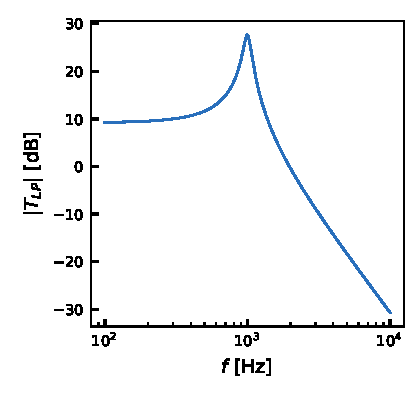
\includegraphics[clip, width=0.37\columnwidth]{./fig/LPF_amp.pdf}}%
    \hspace{5truemm}
    \subfigure[Phase responses]{%
        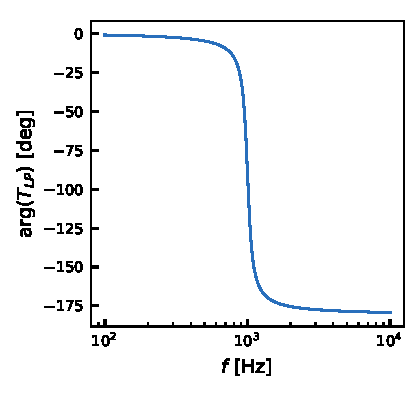
\includegraphics[clip, width=0.37\columnwidth]{./fig/LPF_arg.pdf}}%
    \end{center}
    \caption{Graphs of theoretical values of magnitude and phase characteristics in LPF ($Q$=8.4, $f_0$ = 1000[Hz])}
    \label{fig:LPF_graph}
\end{figure}

\subsection{弛張発振器の発振周波数}
Fig.\ref{fig:Relaxation_Oscillator}に弛張発振器の回路図を示す.
\begin{figure}[H]
    \centering
    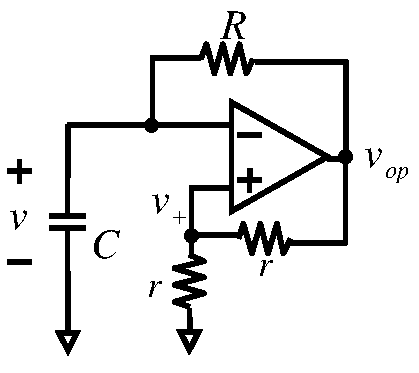
\includegraphics[scale=0.5]{./fig/Relaxation_Oscillator.pdf}
    \caption{Relaxation Oscillator}
    \label{fig:Relaxation_Oscillator}
\end{figure}

 この時,オペアンプと抵抗 $r$ で構成されている回路をはヒステリシス比較器という.Fig.\ref{fig:Hysteresis_comparator}にヒステリシス比較器の回路を示す.\\
 この回路は飽和領域で考える.$v_{d}=v_{+}-v_{i n}>0$ の時は,$v_{o}=E_{s a t}$ であるので,$v_{+}=\frac{E_{\text {sat}}}{2}$ である.ここで,$v_{i n}>\frac{E_{s a t}}{2}$ となると $v_{d}<0$ となり,$v_{o}$ は $E_{sat}$ から$-E_{sat}$ へと切り替わる.同様に $v_{d}>0$ の時は $v_{i n}<-\frac{E_{s a t}}{2}$ となると $v_o$ は $-E_{sat}$ から $E_{sat}$ へ切り替わる.\\
\begin{figure}[H]
    \centering
    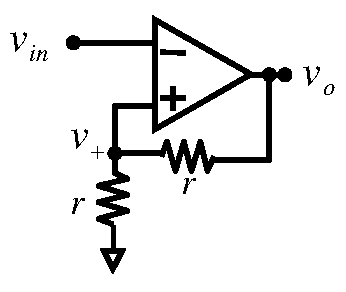
\includegraphics[scale=0.5]{./fig/Hysteresis_comparator.pdf}
    \caption{Hysteresis comparator}
    \label{fig:Hysteresis_comparator}
\end{figure}

 これを踏まえると,Fig.\ref{fig:Relaxation_Oscillator}の弛張発振器回路におけるキャパシタ電圧 $v$ の時間波形はFig.\ref{fig:A_time-domain_waveform_of_the_capacitor_voltage}のようになる.
\begin{figure}[H]
    \centering
    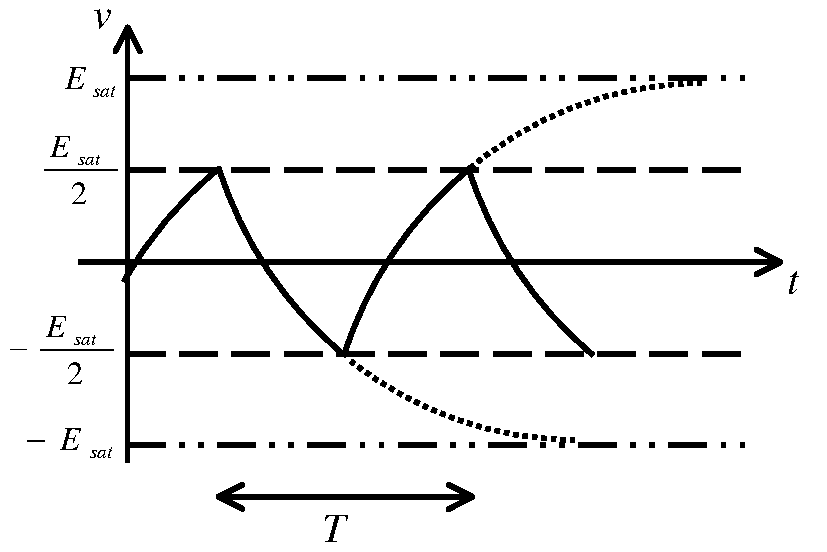
\includegraphics[scale=0.5]{./fig/A_time-domain_waveform_of_the_capacitor_voltage.pdf}
    \caption{A time-domain waveform of the capacitor voltage}
    \label{fig:A_time-domain_waveform_of_the_capacitor_voltage}
\end{figure}

 この時,$-\frac{E_{s a t}}{2}$ から $\frac{E_{s a t}}{2}$ へと変化する電圧は時間の関数としてEqn.(\ref{eqn:RelaxationOscillator})で表現される.
\begin{equation}
    v(t)=\left(v(0)-E_{s a t}\right) e^{-\frac{1}{R C} t}+E_{s a t}
    \label{eqn:RelaxationOscillator}
\end{equation}

 ここに境界条件$v\left(\frac{T}{2}\right)=\frac{E_{s a t}}{2}$ ,$v(0)=\frac{-E_{s a t}}{2}$を代入すると,次の式が得られる.
\begin{equation}
    f = \frac{1}{2 R C \ln 3}
    \label{eqn:RelaxationOscillator_f}
\end{equation}


% 実験手段,測定系の概要,測定装置の名称・型番等を書くこと.また,装置の精度・仕様等の情報もできる限り示すこと.(レポート用紙2枚程度)
\section{実験方法 Experiment}
\subsection{2次低域通過フィルタ}
 与えられた設計仕様は $Q$ = 8.4,$f_0$ = 1000Hz であった.実験で使用する素子は,E24系列の抵抗と 3.3nF,4.7nF,6.8 nFのコンデンサである.この中から,$Q$ と $f_0$ の誤差が最小となる素子の値をEqn.(\ref{eqn:LPF_Q}),Eqn.(\ref{eqn:LPF_omega})もとに総当たりで調べるプログラムを作成した.その結果,$R_g$ = 3.3$\Omega$,$R_f$ = 6.2$\Omega$,$R$ = 24k$\Omega$,$C$ = 6.8nFが最適であると判断した.

\subsection{弛張発振器}
 与えられた設計仕様は $f$ = 1000Hz であった.実験で使用する素子は,E24系列の抵抗と 47nF のコンデンサである.この中から2次LPFの時と同様に$f$ の誤差が最小となる素子の値をプログラムにより,総当たりで調べた.その結果,最適な素子の値は $R$ = 10k$\Omega$,$C$ = 47nF であると判断した.

% % 各自の実験目的に沿った結果を簡潔にまとめること.その他の試行錯誤的実験データは Appendix にまとめる.枚数は各教員の指示に従ってください.(レポート用紙の枚数は教員の指示に従う)
% \section{実験結果 Results}

% % 各自の目的と照らし合わせ,測定結果の妥当性や数値計算結果との整合性などについて考察する.実験結果とサブテキスト/参考書の図式とを比較し議論すること.課題が与えられているテーマに関してはそれについても考察すること.(レポート用紙2枚程度)
% \section{考察 Discussion}

% % 君自身が実験を通じて(実験の方法,まとめ方などで)工夫した点をまとめる.(100字程度 )
% \section{工夫した点}

% 実験結果の羅列ではなく,考察した結果をまとめること.(250字程度)
\section{結論 Conclusion}
 このレポートでは2次低域通過フィルタと弛張発振器について与えられた仕様に即した回路設計を理論に行った.2学期の実験では今回算出した素子の値を元に実際に回路を作成し,動作試験を行う.


% % レポートで引用した参考文献のリストを付ける.
% \section{参考文献 Reference}
% \begin{thebibliography}{9}
%     \bibitem{shinzui_single} 電気の神髄. 単相全波整流回路(単相ブリッジ整流回路). \url{https://denki-no-shinzui.com/12544/}, (参照:2020-05-16)
%     \bibitem{shinzui_three} 電気の神髄. 三相全波整流回路(三相ブリッジ整流回路). \url{https://denki-no-shinzui.com/12978/}, (参照:2020-05-16)
%     \bibitem{denkikigairon} 深尾正 (2015). 電気機器概論. 実教出版株式会社.
% \end{thebibliography}


% % 周辺の関連調査事項,作成プログラムリスト,試行錯誤的実験データ
% \appendix
% \section{Appendix}

\end{document}
